\section{How much depends on the absolute heading?}
\label{sec:heading}

The reviews ask why the output is expressed in ENU although an image pair cannot observe north, how accurate the learned heading is and whether it generalises, and whether the baselines of Table~2 fail only because of this frame. This section answers the three questions. In short: every number that involves $\Delta x$ and $\Delta y$ in ENU depends on a heading prior that is accurate on PairUAV only because the surroundings of the test buildings were seen in training; the camera-frame results do not depend on it; and the baselines do not fail because of the frame.

\subsection{Two frames}
\label{sec:frames}

An image pair determines the displacement in the frame of the source camera. DreamNav estimates it in the levelled frame of that camera (\cref{sec:conv}), and rotates the horizontal part into ENU, the frame of the labels and of Tables~2 and~3, with an absolute heading that two networks predict from the images (\cref{sec:absh}). The application does not need this rotation: the closed loop of Sec.~5.4 executes the estimate in the camera frame and never uses the absolute heading (\cref{sec:tablefive}), and an aircraft reads its heading from its compass.

\begin{table}[t]
\centering
\caption{\textbf{What the heading costs in the pose output.} Same estimates, expressed in the camera frame or rotated into ENU with different sources of the absolute heading; the compass rows add Gaussian noise to the true heading. Horizontal MAE and EPE in metres.}
\label{tab:heading_cost}
\footnotesize
\setlength{\tabcolsep}{3pt}
\resizebox{\columnwidth}{!}{%
\begin{tabular}{@{}lcccc@{}}
\toprule
& Coarse & \multicolumn{3}{c}{Refined} \\
\cmidrule(lr){2-2}\cmidrule(lr){3-5}
Frame and heading source & \SRe & $\Delta x$ / $\Delta y$ & EPE med. & \SRe \\
\midrule
Camera frame (no heading) & 59.9 & 0.46 / 0.50 & 0.53 & 78.7 \ci{77.0}{80.2} \\
ENU, learned heading (paper) & 44.3 & 0.99 / 0.98 & 0.76 & 61.9 \ci{58.9}{64.9} \\\midrule
ENU, compass, $\sigma{=}1^\circ$ & 58.6 & 0.52 / 0.53 & 0.58 & 77.7 \\
ENU, compass, $\sigma{=}2^\circ$ & 53.7 & 0.58 / 0.59 & 0.69 & 72.5 \\
ENU, compass, $\sigma{=}5^\circ$ & 35.9 & 0.82 / 0.84 & 1.02 & 49.0 \\
ENU, compass, $\sigma{=}10^\circ$ & 21.8 & 1.29 / 1.30 & 1.57 & 29.5 \\
\bottomrule
\end{tabular}}
\end{table}

\begin{table}[t]
\centering
\caption{\textbf{Error of the absolute-heading prior} on the 6{,}364 test pairs (degrees; heading of the source view, wrapped absolute error).}
\label{tab:heading_err}
\footnotesize
\setlength{\tabcolsep}{3pt}
\resizebox{\columnwidth}{!}{%
\begin{tabular}{@{}lccccc@{}}
\toprule
Estimator & Mean & Median & P90 & $>10^\circ$ (\%) & $>45^\circ$ (\%) \\
\midrule
Raw-view network, one image & 6.71 \ci{5.12}{8.62} & 1.97 & 12.8 & 13.7 & 2.4 \\
Nadir-rectified network, one image & 6.49 \ci{4.92}{8.50} & 1.59 & 12.1 & 12.0 & 2.8 \\
Coarse stage: raw-view, both images & 5.75 \ci{4.07}{7.66} & 1.64 & 10.7 & 11.0 & 1.9 \\
Refined stage: both networks, both images & 5.31 \ci{3.61}{7.33} & 1.31 & 9.6 & 9.6 & 1.9 \\
\bottomrule
\end{tabular}}
\end{table}


\Cref{tab:heading_cost} expresses the same estimates in the two frames. The range error, $\Delta z$, $\dth$ and $\dpsi$ do not depend on the heading; $\Delta x$, $\Delta y$ and the endpoint error do. The endpoint success of the refined stage is \hdCamSRe\% in the camera frame and \hdEnuSRe\% in ENU with the learned heading, and \hdFailFixed\% of the ENU failures succeed with the true heading. With the true heading perturbed by Gaussian noise, as a compass would give it, the success is \hdCompOneSRe\% for $\sigma{=}1^\circ$, \hdCompTwoSRe\% for $2^\circ$ and \hdCompFiveSRe\% for $5^\circ$: at a mean horizontal displacement of 11\,m, one metre corresponds to $5^\circ$. On this test set the learned prior is thus worth a compass with an error between $2^\circ$ and $5^\circ$. The camera-frame numbers should be the primary result, with the ENU numbers reported for a stated heading source.

\subsection{Error of the heading prior}
\label{sec:headerr}

\Cref{tab:heading_err} gives the error that the main paper does not report. After fusion over the two images and the two networks the mean error is $\hdSiiMean^\circ$ and the median $\hdSiiMed^\circ$; the distribution has a heavy tail, with \hdSiiGtTen\% of the pairs above $10^\circ$ and \hdSiiGtFortyFive\% above $45^\circ$. The error is mostly a bias shared by the images of a building, not image noise: removing the mean error of each building leaves $\hdNoiseOnly^\circ$ of mean error, the building biases alone account for $\hdBiasOnly^\circ$, and five buildings contribute \hdTopFiveShare\% of the total. The predicted concentration is informative: discarding the 5\% least confident pairs lowers the mean error to $\hdCovMae^\circ$ and the share above $45^\circ$ to \hdCovGtFortyFive\%.

\begin{figure*}[t]
\centering
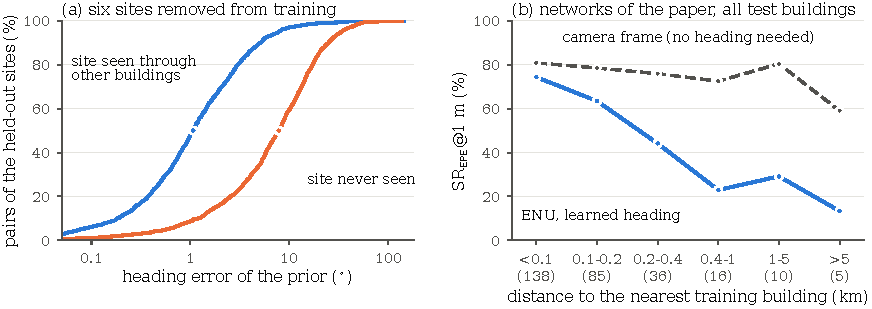
\includegraphics[width=0.92\textwidth]{figures/fig_heading.pdf}
\caption{\textbf{The heading prior depends on having seen the site.} (a) Cumulative distribution of the heading error on the test pairs of six sites, for the raw-view network of the paper, which saw other buildings of these sites during training, and for the same network re-trained without them; dots mark the medians. (b) Endpoint success of the refined stage against the distance from the test building to the nearest training building, in ENU with the learned heading and in the camera frame; the number of test buildings is given in parentheses.}
\label{fig:heading}
\end{figure*}

\begin{table}[t]
\centering
\caption{\textbf{Heading prior on sites that were never seen.} Raw-view heading network re-trained after removing every building of six sites from its training set; estimates of the refined stage rotated into ENU with the fused heading of this network. Heading error in degrees.}
\label{tab:heading_site}
\footnotesize
\setlength{\tabcolsep}{3pt}
\resizebox{\columnwidth}{!}{%
\begin{tabular}{@{}lccccc@{}}
\toprule
& \multicolumn{3}{c}{Heading error} & EPE med. & \SRe, ENU \\
\cmidrule(lr){2-4}
Heading network & mean & med. & $>10^\circ$ (\%) & (m) & (\%) \\
\midrule
\multicolumn{6}{@{}l}{\emph{Held-out sites} (84 test buildings, 1{,}852 pairs; camera frame: 78.4\% \SRe)}\\
\quad paper network & 2.4 \ci{1.7}{3.2} & 1.1 & 3.0 & 0.73 & 67.5 \ci{63.3}{71.9} \\
\quad re-trained without the six sites & 11.2 \ci{9.4}{13.1} & 7.8 & 40.6 & 1.78 & 27.4 \ci{22.4}{32.5} \\
\midrule\multicolumn{6}{@{}l}{\emph{Other sites} (206 test buildings, 4{,}512 pairs; camera frame: 78.8\% \SRe)}\\
\quad paper network & 7.1 \ci{4.9}{10.1} & 2.0 & 14.2 & 0.89 & 55.4 \ci{51.3}{58.9} \\
\quad re-trained without the six sites & 6.5 \ci{4.9}{8.5} & 2.4 & 16.6 & 0.96 & 51.8 \ci{47.9}{55.3} \\
\bottomrule
\end{tabular}}
\end{table}


\subsection{Dependence on the training sites}
\label{sec:headsite}

The test buildings are held out, but their surroundings are not. The buildings of PairUAV are grouped in campuses, and the median test building stands \hdDistMedian\,m from a training building (90th percentile \hdDistPNinety\,m), less than the width of the ground footprint of one image. \Cref{fig:heading}(b) shows the consequence. For the \hdDistAN{} test buildings within 100\,m of a training building the median heading error is $\hdDistAMed^\circ$ and the ENU success \hdDistAEnu\%; between 0.4 and 1\,km they are $\hdDistDMed^\circ$ and \hdDistDEnu\%; for the \hdDistFN{} buildings farther than 5\,km, $\hdDistFMed^\circ$ and \hdDistFEnu\%. The camera-frame success stays between \hdDistDCam\% and \hdDistACam\% up to 5\,km; its lower value for the last \hdDistFN{} buildings (\hdDistFCam\%) has an interval of \ci{\sgZeroSReLo}{\sgZeroSReHi} and is not significant. Over all test buildings the camera-frame success is unrelated to the number of training buildings of the site (Spearman \sgRho).

To measure the prior on sites that were never seen, we re-train the raw-view network after removing all \hdSdRemoved{} training buildings of \hdSdSites{} sites, which contain \hdSdBuildings{} test buildings (\cref{tab:heading_site}, \cref{fig:heading}(a)). On these sites the median heading error rises from $\hdSdSeenMed^\circ$ to $\hdSdUnseenMed^\circ$ and the ENU endpoint success falls from \hdSdSeenSRe\% to \hdSdUnseenSRe\%, a paired difference of \hdSdDelta{} points \ci{\hdSdDeltaLo}{\hdSdDeltaHi}; the camera-frame success on the same pairs is \hdSdCamSRe\%. On the other sites the re-trained network changes the success by \hdSdOtherDelta{} points \ci{\hdSdOtherDeltaLo}{\hdSdOtherDeltaHi}, which is the effect of the smaller training set alone. On an unseen site the error is close to one constant offset for the whole site, between $\hdSdOffMin^\circ$ and $\hdSdOffMax^\circ$ for the six sites, with a resultant length of the signed errors of \hdSdResLo{} to \hdSdResHi. Three limitations apply: only the raw-view network was re-trained, so both rows of \cref{tab:heading_site} use one network instead of two; there is one split and one seed; and a control with the same number of training buildings removed elsewhere was not trained to convergence.

The ENU results of Tables~2 and~3 therefore hold for test buildings that stand next to training buildings. They should not be read as results on unseen scenes, and the statement of the abstract on this point is corrected in \cref{sec:corrections}.

\begin{table}[t]
\centering
\caption{\textbf{What the heading prior reads.} Error of the heading predicted from one image (both networks) after an image operation, on 2{,}000 test images (degrees). $^\dagger$raw-view network only; a zoom of 3.6 corresponds to the flight height of the real photographs.}
\label{tab:heading_sens}
\footnotesize
\setlength{\tabcolsep}{3pt}
\resizebox{\columnwidth}{!}{%
\begin{tabular}{@{}lccc@{}}
\toprule
Operation on the image & Mean & Median & $>45^\circ$ (\%) \\
\midrule
None & 6.5 & 1.7 & 3 \\
\midrule Brightness $\times0.6$, $\times1.4$ & 6.9, 7.1 & 1.8, 1.9 & 3, 3 \\
Contrast $\times0.6$, $\times1.4$ & 7.3, 7.0 & 1.9, 2.0 & 3, 3 \\
Gamma 0.6, 1.6 & 8.8, 8.8 & 3.3, 2.7 & 3, 4 \\
Shadows lifted & 7.7 & 2.0 & 3 \\
Tiles of 64, 32 px shuffled & 10.0, 16.5 & 4.0, 7.6 & 4, 8 \\
\midrule Blur, $\sigma{=}1$, 2 px & 9.0, 21.7 & 3.1, 9.8 & 4, 14 \\
JPEG, quality 20 & 26.5 & 12.2 & 18 \\
Grey levels only & 43.5 & 35.7 & 39 \\
Hue rotated by $90^\circ$, $180^\circ$ & 39.1, 88.6 & 19.6, 89.6 & 29, 69 \\
Luminance inverted, colour kept & 91.9 & 93.5 & 72 \\
Negative image & 135.4 & 156.0 & 91 \\
\midrule Centre zoom $\times1.5$, $\times2$, $\times3.6^\dagger$ & 10.8, 16.0, 33.7 & 4.0, 6.4, 16.7 & 4, 8, 23 \\
\bottomrule
\end{tabular}}
\end{table}


\subsection{What the prior reads}
\label{sec:headsens}

\Cref{tab:heading_sens} applies image operations to \hdSensN{} test images. Global changes of brightness, contrast and gamma, lifting the shadows, and even shuffling tiles of 64 pixels leave the prediction almost unchanged: the cue is local, not the layout of the scene. Removing the colour (median error $\hdSensGray^\circ$), rotating the hue ($\hdSensHue^\circ$ for $180^\circ$), strong compression ($\hdSensJpeg^\circ$) and blur degrade it severely, and on the negative image \hdSensNegFlip\% of the predictions turn by $180^\circ$. A change of scale by 3.6, that of the real photographs, gives a median error of $\hdSensZoom^\circ$. For the \hdSouthN{} test buildings of the southern hemisphere the median error is $\hdSouthErr^\circ$. These observations are consistent with a cue tied to the direction of the illumination, such as the shadows, whose relation to north is fixed for the imagery of a site and reverses in the southern hemisphere. We have not verified this interpretation directly: the dataset has one rendering per site, so the illumination cannot be varied in a controlled way. Whatever the cue, it is a property of the imagery from which PairUAV is rendered and not of the scene.

On the real photographs the prior does not transfer: the median error is $\hdRealOneMed^\circ$ from one image and $\hdRealFusedMed^\circ$ after fusion, where chance is $90^\circ$, and the ENU endpoint success is \hdRealEnuSRe\% against \hdRealCamSRe\% in the camera frame (\cref{sec:real}). The failure is at least detectable: the median concentration predicted by the raw-view network falls from \hdRenderKappa{} on the rendered test images to \hdRealKappa{} on the photographs.

\begin{table}[t]
\centering
\caption{\textbf{Baselines of Table~2 re-trained with the horizontal target in the camera frame} (same recipes; 6{,}364 test pairs). Hor.: mean absolute error of the two horizontal components; Corr.: correlation between predicted and true horizontal components, averaged over the two. A number in parentheses: recipes repeated with that many seeds, mean reported. $\pi_{0.5}$ and $\pi_0$-FAST were not re-trained.}
\label{tab:camframe}
\footnotesize
\setlength{\tabcolsep}{2.5pt}
\resizebox{\columnwidth}{!}{%
\begin{tabular}{@{}lcccccccccc@{}}
\toprule
& \multicolumn{2}{c}{$d$ (m)} & \multicolumn{2}{c}{\SRd{} (\%)} & \multicolumn{2}{c}{Hor. (m)} & \multicolumn{2}{c}{Corr.} & \multicolumn{2}{c}{EPE med. (m)} \\
\cmidrule(lr){2-3}\cmidrule(lr){4-5}\cmidrule(lr){6-7}\cmidrule(lr){8-9}\cmidrule(lr){10-11}
Training target & ENU & cam. & ENU & cam. & ENU & cam. & ENU & cam. & ENU & cam. \\
\midrule
ViNT & 18.91 & 18.40 & 0.3 & 0.2 & 7.46 & 7.26 & $-0.01$ & $+0.02$ & 20.0 & 20.1 \\
NoMaD & 7.14 & 7.08 & 8.6 & 8.6 & 9.62 & 9.57 & 0.00 & $+0.01$ & 25.2 & 25.1 \\
DINO-WM (2) & 10.33 & 10.27 & 6.1 & 6.1 & 8.94 & 8.87 & $-0.01$ & $-0.01$ & 23.6 & 23.7 \\
Visual Foresight & 10.30 & 10.28 & 5.7 & 5.7 & 8.73 & 8.54 & $-0.01$ & $+0.01$ & 23.0 & 22.9 \\
DINOv3 ViT-7B (5) & 12.86 & 13.05 & 3.1 & 3.0 & 7.83 & 7.57 & $+0.01$ & $+0.02$ & 19.2 & 19.1 \\
Sample4Geo (5) & 11.00 & 10.30 & 5.1 & 5.7 & 8.29 & 8.58 & $+0.01$ & $+0.01$ & 21.0 & 21.7 \\
\midrule
Regression on MASt3R statistics & 5.40 & 3.15 & 9.9 & 21.5 & 7.44 & 3.68 & $+0.07$ & $+0.83$ & 12.2 & 6.1 \\
\midrule
No motion & 20.32 & 20.32 & 0.0 & 0.0 & 7.45 & 7.26 & -- & -- & 20.2 & 20.2 \\
\bottomrule
\end{tabular}}
\end{table}


\subsection{Do the baselines fail because of the frame?}
\label{sec:camframe}

One review suspects that the baselines of Table~2 fail mainly because they must regress $\Delta x$ and $\Delta y$ in ENU. We re-trained six of the eight with the horizontal target in the camera frame, with otherwise the recipes of Table~2 (\cref{sec:baselines}); $\pi_{0.5}$ and $\pi_0$-FAST could not be re-trained on the shared GPU. \Cref{tab:camframe} shows no effect. In both frames the horizontal error of every re-trained baseline is at or above that of predicting no motion (\cfZeroCamHor\,m), the correlation between its predicted and the true horizontal displacement is at most \cfMaxCamCorr, its endpoint success at 1\,m is at most \cfMaxCamSRe\%, and its \SRd{} (at most \cfMaxCamSRd\%) is at the level of a constant distance equal to the training median (\cfConstSRd\%). These models do not perceive the displacement at all; the frame of the target is not what limits them. Three diagnostics support this. ViNT and NoMaD receive inputs of $85{\times}64$ and $96{\times}96$ pixels, in which one metre on the ground is half a pixel. Heads trained to convergence on the frozen DINOv3 and Sample4Geo descriptors stay at the level of no motion in both frames. For the two world models the planning cost changes by less than 0.1\% when the horizontal displacement of the action is exchanged with that of another pair.

The concern is nevertheless justified for a model that does perceive the displacement. The regression on pooled MASt3R statistics, which is the prior branch of DreamNav, improves from \cfMlpEnuD\,m to \cfMlpCamD\,m of range error and from \cfMlpEnuSRd\% to \cfMlpCamSRd\% \SRd{} when its target is expressed in the camera frame, and the correlation of its horizontal prediction with the truth from \cfMlpEnuCorr{} to \cfMlpCamCorr. For this reason all results of this document are given in the camera frame, and \cref{tab:main_metrics} gives both frames for our method.
